\documentclass[conference]{IEEEtran}
\usepackage{tabularx}
\usepackage{fixltx2e}
\usepackage[backend=bibtex]{biblatex}
\usepackage{graphicx}
\usepackage{multicol}
\graphicspath{ {images/} }
\bibliography{assignment_4}


% correct bad hyphenation here
\hyphenation{op-tical net-works semi-conduc-tor}


\begin{document}
\raggedbottom

%
% paper title
% Titles are generally capitalized except for words such as a, an, and, as,
% at, but, by, for, in, nor, of, on, or, the, to and up, which are usually
% not capitalized unless they are the first or last word of the title.
% Linebreaks \\ can be used within to get better formatting as desired.
% Do not put math or special symbols in the title.
\title{Assignment \#4}
% author names and affiliations
% use a multiple column layout for up to three different
% affiliations
\author{\IEEEauthorblockN{SwagMasterFlex}
\IEEEauthorblockA{Department of Electrical and Computer Engineering\\
University of British Columbia\\
Vancouver, Canada\\
}
}


% make the title area
\maketitle

\section{Question \#1}

\noindent\textbf{Student \#:}\\
\texttt{33657115}
\\\\
\textbf{Hash:}\\
\texttt{LTF6A2CBE86F0354722C9B377E9E187885D1DE6B5D}\\\\
\textbf{Bits of entropy}\\
\texttt{$\sim$13 bits = $ln(10^4)/ln(2)$}\\\\
\textbf{Password found:}\\
\texttt{1531}\\\\
\textbf{CPU/GPU time spent:}\\
Less than a second
\\\\

I started off by examining the number of characters in the hashed password. The count came out to 42 characters (168 bits), which didn't match any of the common hashing algorithms. Next, I observed that the first two characters of my hash were non-hex, while the other 40 characters were hex characters.\\

This led me believe that the first two characters of the hash were stored as the salt, and the following 40 characters were the result of hashing the password using \textbf{SHA1}, since \textbf{SHA1} produces a 20-character hash (40-character hex-representation). \\

To crack the password, I ran \textbf{oclHashcat} \cite{oclHashcat}, a password cracker that runs on the GPU. It took less than a second for \textbf{oclHashcat} to crack the password.\\\\

\newpage

\section{Question \#2}
\noindent\textbf{Student \#:}\\
\texttt{33657115}
\\\\
\textbf{Hash:}\\
\texttt{CS0DF2939D499DCC46A693653DB281FDBB016B502B}\\\\
\textbf{Bits of entropy}\\
\texttt{$\sim$37 bits = $ln(76^6)/ln(2)$}\\\\
\textbf{Password found:}\\
\texttt{y\%jtqf}\\\\
\textbf{CPU/GPU time spent:}\\
3 mins, 30 secs\\
(70,748,995,584 combinations tried)
\\\\

Since the format of the hash is the same as \texttt{Question \#1}, I made the same assumption as before. Namely, that the hash function used to hash the password was \textbf{SHA1}.\\

Again, I ran \textbf{oclHashcat} in order to crack the password. It took the program about three and a half minutes to find the password.

\newpage

\section{Question \#3}
\noindent\textbf{Student \#:}\\
\texttt{33657115}
\\\\
\textbf{Found Password:}\\
\texttt{\#l!Je$*$iDiHBbB5O\#\_Bm}\\\\

In order to begin, I disassembled the binary using \textbf{IDAPro} \cite{IDAPro}. This allowed me to step through the assembly code in order to find the password.\\

The first thing I noticed was that the program was denying access if the length of the string was not nineteen characters (\texttt{0x13}) long. Next, I inputted a nineteen-character long password, which allowed me to progress further through the code. 

\begin{figure}[h]
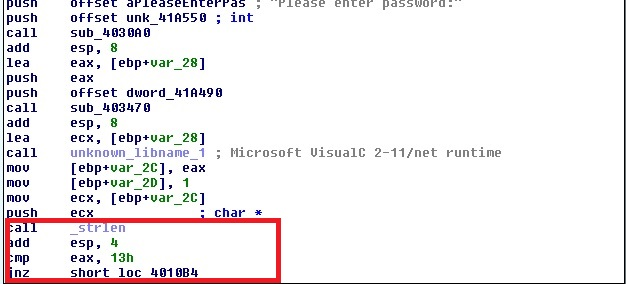
\includegraphics[width=\columnwidth]{image1.jpg}
\caption{Result of \texttt{strlen()} being compared with \texttt{0x13}}
\centering
\end{figure}\mbox{}

At this point, I noticed that the program was fetching one character at a time from my inputted password string and offset \texttt{0x419051}, and comparing these two values. I assumed that this was the password that the program was looking for. I extracted 19 characters from this offset location, and inputted this result on the next program iteration. This password finally granted me access.\\

\begin{figure}[!h]
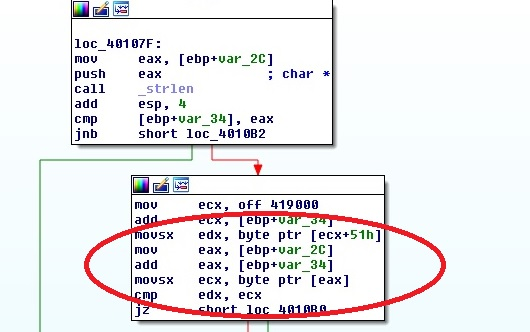
\includegraphics[width=\columnwidth]{image2.jpg}
\caption{My input string being compared with the stored password}
\centering
\end{figure}\mbox{}

In order to patch the program, I changed the value of \texttt{\%ebp $+$ var\_2D} to always be \texttt{1}, indicating that the correct password was entered. When the value of \texttt{\%ebp $+$ var\_2D} was tested (or compared to \texttt{0}), it would always pass through, and grant me access.\\

\begin{figure}[h]
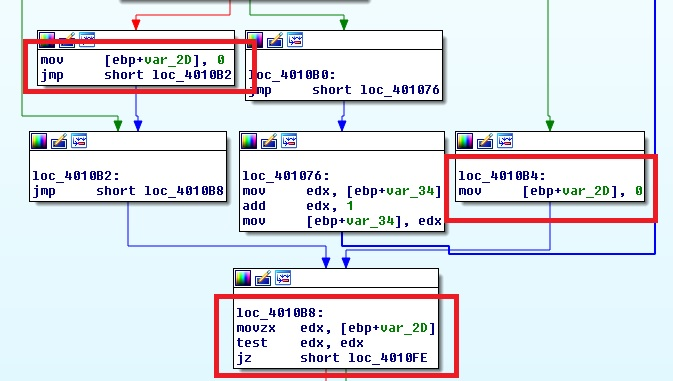
\includegraphics[width=\columnwidth]{image3.jpg}
\caption{Assigning \texttt{\%ebp $+$ var\_2D} to \texttt{1} prevents the program from jumping to the \texttt{"Access Denied"} block}
\centering
\end{figure}\mbox{}

\newpage

\section{Question \#4}
\noindent\textbf{Student \#:}\\
\texttt{33657115}\\\\
\textbf{Hash:}\\
\texttt{929a2e98651FD2DDE3629F8DB8F0BDC32B673BE4}\\\\
\textbf{Found Password:}\\
\texttt{M7rUAV}\\\\
\textbf{CPU/GPU time spent:}\\
2 mins, 53 secs\\\\

The process to find the required password for this problem was very similar to \texttt{Question \#3}. Once again I used \textbf{IDAPro}. The presence of a \textbf{SHA1} function led me to believe that password was stored as a hash. The only parameter to the \textbf{SHA1} function was the input password itself, which led me to assume that no salt was used to hash the password.\\

\begin{figure}[h]
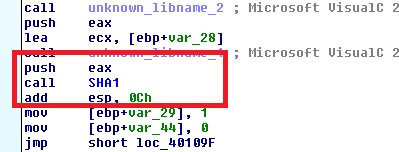
\includegraphics[width=\columnwidth]{image4.jpg}
\caption{\texttt{SHA1} function shown with parameters (notice no salt passed)}
\centering
\end{figure}\mbox{}

I noticed that my hashed input string was being compared with a string located at \texttt{0x4141F3}. I extracted 20 characters from this location and took it to be the password hash. Next, I entered the hash into \textbf{oclHashcat} and it generated the corresponding plaintext password.\\

\begin{figure}[h]
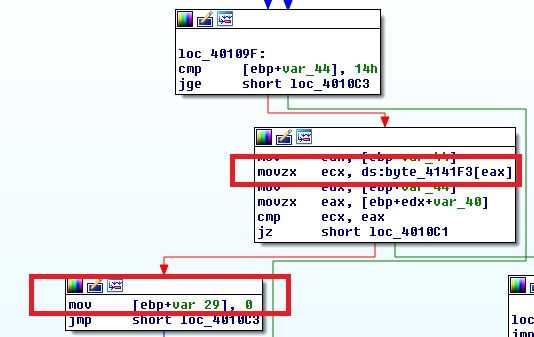
\includegraphics[width=\columnwidth]{image5.jpg}
\caption{My hashed input being compared with the hashed password. Also shows the instruction that I patched}
\centering
\end{figure}\mbox{}\\

To patch the program, I changed the value of \texttt{\%ebp $+$ var\_29} to always be \texttt{1}. \textbf{Fig. 5} highlights where I changed the value of this variable from \texttt{0} to \texttt{1}. This allowed the program to always grant access, regardless of whether the password was correct or not.\\

In order to allow the user to change the password of the program, I created a Python program that asked the user for the new password, hashed it, and then overwrote the old hashed password, which was stored in static memory in the binary, with the new hashed password. The next time the user ran the program, they would need to enter the new password in order to gain access.\\\\

\printbibliography

%
% For peerreview papers, this IEEEtran command inserts a page break and
% creates the second title. It will be ignored for other modes.
\IEEEpeerreviewmaketitle


% that's all folks
\end{document}


